\documentclass[11pt,a4paper]{article}

\usepackage[utf8]{inputenc}
\usepackage[T1]{fontenc}
\usepackage{amsmath, amssymb}
\usepackage{enumitem}
\usepackage{graphicx}
\usepackage{geometry}
\usepackage{mathtools}
\usepackage{physics}
\usepackage{xcolor}
\usepackage{array}
\usepackage{subcaption}


\geometry{margin=2.5cm}

\title{Double pendule}
\author{Favre Florian}
\date{18.01.2025}

\begin{document}

\maketitle

\section{Schéma}

\begin{figure}[h!]
    \centering
    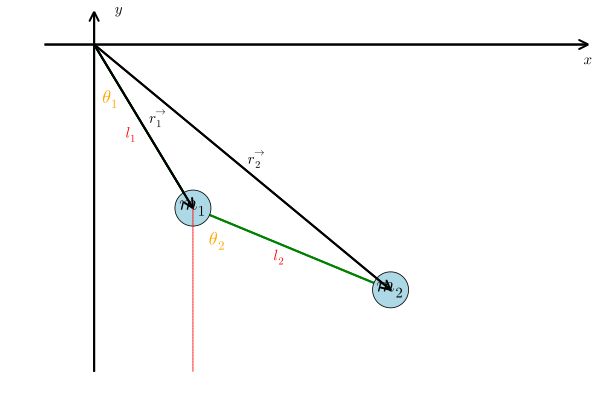
\includegraphics[width=0.7\textwidth]{img/shema_double_pendule.jpg}
    \caption{Schéma du double pendule}
\end{figure}

\section{Paramètres du système}
\begin{itemize}[leftmargin=*]
    \item Masse du premier pendule : $m_1$ [kg]
    \item Masse du deuxième pendule : $m_2$ [kg]
    \item Longueur de la tige du premier pendule : $L_1$ [m]
    \item Longueur de la tige du deuxième pendule : $L_2$ [m]
    \item Angle du premier pendule (sens anti-horaire) : $\theta_1$ [rad]
    \item Angle du deuxième pendule (sens anti-horaire) : $\theta_2$ [rad]
    \item Vitesse angulaire du premier pendule : $\omega_1$ [rad/s]
    \item Vitesse angulaire du deuxième pendule : $\omega_2$ [rad/s]
    \item Accélération angulaire du premier pendule : $\alpha_1$ [rad/s$^2$]
    \item Accélération angulaire du deuxième pendule : $\alpha_2$ [rad/s$^2$]
    \item Constante gravitationnelle : $g = 9{,}81$ [m/s$^2$]
\end{itemize}

\section{Équations}

\subsection{Positions}

\begin{align}
\frac{x_1}{l_1} &= \sin(\theta_1) \\ 
x_1 &= l_1 \sin(\theta_1) \\\\
\frac{y_1}{l_1} &= \cos(\theta_1) \\
y_1 &= -l_1 \cos(\theta_1) \\\\
x_2 &= x_1 + l_2 \sin(\theta_2) \\
x_2 &= l_1 \sin(\theta_1) + l_2 \sin(\theta_2) \\\\
y_2 &= y_1 - l_2 \cos(\theta_2) \\
y_2 &= -l_1 \cos(\theta_1) - l_2 \cos(\theta_2)
\end{align}

\subsubsection{Résumé}

\begin{align}
x_1(t) &= l_1 \sin(\theta_1(t)) \\
y_1(t) &= -l_1 \cos(\theta_1(t)) \\
x_2(t) &= l_1 \sin(\theta_1(t)) + l_2 \sin(\theta_2(t)) \\
y_2(t) &= -l_1 \cos(\theta_1(t)) - l_2 \cos(\theta_2(t))
\end{align}

\subsection{Vitesse}

\begin{align}
v_{x1} &= \frac{dx_1}{dt} = l_1 \cos(\theta_1(t))\dot{\theta}_1(t) \\
v_{y1} &= \frac{dy_1}{dt} = -l_1 \sin(\theta_1(t))\dot{\theta}_1(t) \\
v_{x2} &= l_1 \cos(\theta_1(t))\dot{\theta}_1(t) + l_2 \cos(\theta_2(t))\dot{\theta}_2(t) \\
v_{y2} &= -l_1 \sin(\theta_1(t))\dot{\theta}_1(t) - l_2 \sin(\theta_2(t))\dot{\theta}_2(t)
\end{align}

\subsubsection{Résumé}

\begin{align}
v_{x1}(t) &= l_1 \cos(\theta_1(t))\dot{\theta}_1(t) \\
v_{y1}(t) &= -l_1 \sin(\theta_1(t))\dot{\theta}_1(t) \\
v_{x2}(t) &= l_1 \cos(\theta_1(t))\dot{\theta}_1(t)
+ l_2 \cos(\theta_2(t))\dot{\theta}_2(t) \\
v_{y2}(t) &= -l_1 \sin(\theta_1(t))\dot{\theta}_1(t)
- l_2 \sin(\theta_2(t))\dot{\theta}_2(t)
\end{align}

\subsection{Accélération}

\begin{align}
a_{x1}(t) &= -l_1 \sin(\theta_1)\dot{\theta}_1^2
+ l_1 \cos(\theta_1)\ddot{\theta}_1 \\
a_{y1}(t) &= -l_1 \cos(\theta_1)\dot{\theta}_1^2
- l_1 \sin(\theta_1)\ddot{\theta}_1 \\
a_{x2}(t) &= -l_1 \sin(\theta_1)\dot{\theta}_1^2
+ l_1 \cos(\theta_1)\ddot{\theta}_1
- l_2 \sin(\theta_2)\dot{\theta}_2^2
+ l_2 \cos(\theta_2)\ddot{\theta}_2 \\
a_{y2}(t) &= -l_1 \cos(\theta_1)\dot{\theta}_1^2
- l_1 \sin(\theta_1)\ddot{\theta}_1
- l_2 \cos(\theta_2)\dot{\theta}_2^2
- l_2 \sin(\theta_2)\ddot{\theta}_2
\end{align}

\subsection{Forces}

\begin{figure}[h!]
    \centering
    \begin{subfigure}{0.45\textwidth}
        \centering
        \includegraphics[width=0.6\textwidth]{img/Force_m1.png}
        \caption{Forces appliquées à $m_1$}
    \end{subfigure}
    \hfill
    \begin{subfigure}{0.45\textwidth}
        \centering
        \includegraphics[width=0.6\textwidth]{img/Force_m2.png}
        \caption{Forces appliquées à $m_2$}
    \end{subfigure}
    \caption{Schéma des forces du double pendule.\\ Source : https://www.youtube.com/watch?v=SXj1P9Ra5AM}
\end{figure}

Vecteur unitaire pour la direction des forces de tension:
\begin{align}
\vec{u}_1(t) &= 
\begin{pmatrix}
\sin(\theta_1(t)) \\
\cos(\theta_1(t))
\end{pmatrix}, \quad
\vec{u}_2(t) =
\begin{pmatrix}
\sin(\theta_2(t)) \\
\cos(\theta_2(t))
\end{pmatrix} \\\\
\vec{g} &= (0,-g)
\end{align}

Deuxième Loi de Newton, la somme des forces = m$\vec{a}$

\begin{align}
m_1 \vec{a}_1(t) &= -T_1(t)\vec{u}_1(t) + T_2(t)\vec{u}_2(t) + m_1\vec{g} \\
m_2 \vec{a}_2(t) &= -T_2(t)\vec{u}_2(t) + m_2\vec{g}
\end{align}

\subsubsection{Résolution}

On sépare les forces pour l'axe x et l'axe y:
\begin{align}
m_1 a_{x1} &= -T_1 \sin(\theta_1) + T_2 \sin(\theta_2) \\
m_1 a_{y1} &= -T_1 \cos(\theta_1) + T_2 \cos(\theta_2) - m_1 g \\
m_2 a_{x2} &= -T_2 \sin(\theta_2) \\
m_2 a_{y2} &= -T_2 \cos(\theta_2) - m_2 g
\end{align}

On remplace les $a_i$ par les valeurs trouvées pour l'accélération ci-dessus.

\begin{align}
m_1 \left(-l_1 \sin(\theta_1)\dot{\theta}_1^2
+ l_1 \cos(\theta_1)\ddot{\theta}_1\right) &= -T_1 \sin(\theta_1) + T_2 \sin(\theta_2) \\
m_1 \left(-l_1 \cos(\theta_1)\dot{\theta}_1^2
- l_1 \sin(\theta_1)\ddot{\theta}_1\right) &= -T_1 \cos(\theta_1) + T_2 \cos(\theta_2) - m_1 g
\end{align}
\begin{align}
m_2 \left(-l_1 \sin(\theta_1)\dot{\theta}_1^2
+ l_1 \cos(\theta_1)\ddot{\theta}_1
- l_2 \sin(\theta_2)\dot{\theta}_2^2
+ l_2 \cos(\theta_2)\ddot{\theta}_2\right) &= -T_2 \sin(\theta_2) \\
m_2 \left(-l_1 \cos(\theta_1)\dot{\theta}_1^2
- l_1 \sin(\theta_1)\ddot{\theta}_1
- l_2 \cos(\theta_2)\dot{\theta}_2^2 - l_2 \sin(\theta_2)\ddot{\theta}_2\right) &= -T_2 \cos(\theta_2) - m_2 g
\end{align}

\newpage

On isole $T_2$ depuis la 4ème équation

\begin{align}
T_2 &= \frac{m_2(l_1 cos \theta_1 \dot{\theta_1^2}+l_1 cos \theta_2 \dot{\theta_2^2}+l2 sin \theta_2 \ddot{\theta_2}+g)}{cos \theta_2}
\end{align}

On remplace $T_2$ dans la 3ème équation

\begin{align}
\begin{aligned}
m_2 \Big(
&- l_1 \sin(\theta_1)\dot{\theta}_1^2
+ l_1 \cos(\theta_1)\ddot{\theta}_1
- l_2 \sin(\theta_2)\dot{\theta}_2^2
+ l_2 \cos(\theta_2)\ddot{\theta}_2
\Big)
= \\
&\quad
-\frac{m_2}{\cos\theta_2}
\Big(
l_1 \cos\theta_1\,\dot{\theta}_1^2
+ l_2 \cos\theta_2\,\dot{\theta}_2^2
+ l_2 \sin\theta_2\,\ddot{\theta}_2
+ g
\Big)
\sin(\theta_2)
\end{aligned}
\end{align}

On développe les termes.

\begin{align}
\begin{aligned}
&- l_1 \sin(\theta_1)\cos(\theta_2)\,\dot{\theta}_1^2
+ l_1 \cos(\theta_1)\cos(\theta_2)\,\ddot{\theta}_1
- l_2 \sin(\theta_2)\cos(\theta_2)\,\dot{\theta}_2^2 \\
&\quad
+ l_2 \cos^2(\theta_2)\,\ddot{\theta}_2
=
- l_1 \cos(\theta_1)\sin(\theta_2)\,\dot{\theta}_1^2
- l_2 \cos(\theta_2)\sin(\theta_2)\,\dot{\theta}_2^2 \\
&\quad
- l_2 \sin^2(\theta_2)\,\ddot{\theta}_2
- g \sin(\theta_2)
\end{aligned}
\end{align}

On factorise en utilisant les identités trigonométriques

\begin{align}
\begin{aligned}
&l_1 \cos(\theta_1)\cos(\theta_2)\,\ddot{\theta}_1
+ l_2 \big(\cos^2(\theta_2)+\sin^2(\theta_2)\big)\ddot{\theta}_2 \\
&=
l_1 \big(
\sin(\theta_1)\cos(\theta_2)
- \cos(\theta_1)\sin(\theta_2)
\big)\dot{\theta}_1^2
- g \sin(\theta_2)
\end{aligned}
\end{align}

On obtient la première équation

\begin{align}
l_1 \cos(\theta_1-\theta_2)\,\ddot{\theta}_1
+ l_2 \ddot{\theta}_2
=
l_1 \sin(\theta_1-\theta_2)\,\dot{\theta}_1^2
- g \sin(\theta_2)
\end{align}

On utilise la 2ème et 3ème équation pour isoler $T_2 cos \theta_2 $ et $T_2 sin \theta_2$

\begin{align}
    T_2 sin \theta_2 = -m_2 \left(-l_1 \sin(\theta_1)\dot{\theta}_1^2
+ l_1 \cos(\theta_1)\ddot{\theta}_1
- l_2 \sin(\theta_2)\dot{\theta}_2^2
+ l_2 \cos(\theta_2)\ddot{\theta}_2\right)
\end{align}
\begin{align}
    T_2 cos \theta_2 = m_2 \left(l_1 \cos(\theta_1)\dot{\theta}_1^2
+ l_1 \sin(\theta_1)\ddot{\theta}_1
+ l_2 \cos(\theta_2)\dot{\theta}_2^2 + l_2 \sin(\theta_2)\ddot{\theta}_2 + g\right)
\end{align}

On remplace $T_2 sin$ dans la première équation

\begin{align}
\begin{aligned}
    m_1 \left( -l_1 sin \theta_1 \dot{\theta_1^2} + l_1 cos \theta_1 \ddot{\theta_1}\right) x &= -T_1 sin \theta_1 - m_2 (-l_1 sin \theta_1 \dot{\theta_1^2} + l_1 cos \theta_1 \ddot{\theta_1} - l_2 sin \theta_2 \dot{\theta_2^2} + l_2 cos \theta_2 \ddot{\theta_2})
\end{aligned}
\end{align}

On isole $T_1$

\begin{align}
\begin{aligned}
    T_1 = \frac{-m_1(-l_1 sin \theta_1 \dot{\theta_1^2} + l_1 cos \theta_1 \ddot{\theta_1}) - m_2 (-l_1 sin \theta_1 \dot{\theta_1^2} + l_1 cos \theta_1 \ddot{\theta_1} - l_2 sin \theta_2 \dot{\theta_2^2}+l_2 cos \theta_2 \ddot{\theta_2}) }{sin \theta_1}
\end{aligned}    
\end{align}

\newpage

On remplace $T_1$ et $T_2$ dans la deuxième équation

\begin{align}
\begin{aligned}
&m_1 \left(l_1 \cos(\theta_1)\dot{\theta}_1^2
+ l_1 \sin(\theta_1)\ddot{\theta}_1\right) \\
&= \frac{-m_1(-l_1 sin \theta_1 \dot{\theta_1^2} + l_1 cos \theta_1 \ddot{\theta_1}) - m_2 (-l_1 sin \theta_1 \dot{\theta_1^2} + l_1 cos \theta_1 \ddot{\theta_1} - l_2 sin \theta_2 \dot{\theta_2^2}+l_2 cos \theta_2 \ddot{\theta_2}) }{sin \theta_1} \cos(\theta_1)\\
&- m_2 \left(l_1 \cos(\theta_1)\dot{\theta}_1^2
+ l_1 \sin(\theta_1)\ddot{\theta}_1
+ l_2 \cos(\theta_2)\dot{\theta}_2^2 + l_2 \sin(\theta_2)\ddot{\theta}_2 + g\right) - m_1 g
\end{aligned}
\end{align}

On développe les termes

\begin{align}
\begin{aligned}
    &m_1 l_1 cos \theta_1 sin \theta_1 \dot{\theta_1^2} + m_1 l_1 sin^2 \theta_1 \ddot{\theta_1} \\
    &= m_1 l_1 sin \theta_1 cos \theta_1 \dot{\theta_1^2} - m_1 l_1 cos^2 \theta_1 \ddot{\theta_1} + m_2 l_1 cos \theta_1 sin \theta_1 \dot{\theta_1^2} - m_2 l_1 cos^2 \theta_1 \ddot{\theta_1} + m_2 l_2 cos \theta_1 sin \theta_2 \dot{\theta^2_2} \\
    &- m_2 l_2 cos \theta_1 cos \theta_2 \ddot{\theta_2} - m_2 l_1 sin \theta_1 cos \theta_1 \dot{\theta_1^2} - m_2 l_1 sin^2\theta_1 \ddot{\theta_1} - m_2 l_2 sin \theta_1 cos \theta_2 \dot{\theta_2^2} - m_2 l_2 sin \theta_1 sin \theta_2 \ddot{\theta_2}\\
    &- (m_1 + m_2)g sin \theta_1
\end{aligned}
\end{align}

On factorise avec les identités trigonométriques. Et on a donc les 2 équation on l'on peut isolé l'acélération car on a supprimé les tensions.

\begin{align}
l_1 (m_1 + m_2)\ddot{\theta}_1
- m_2 l_2 \cos(\theta_1-\theta_2)\ddot{\theta}_2
=
- (m_1 + m_2) g \sin\theta_1
- m_2 l_2 \sin(\theta_1-\theta_2)\dot{\theta}_2^2
\end{align}



\begin{align}
l_1 \cos(\theta_1-\theta_2)\,\ddot{\theta}_1
+ l_2 \ddot{\theta}_2
=
l_1 \sin(\theta_1-\theta_2)\,\dot{\theta}_1^2
- g \sin(\theta_2)
\end{align}

On pose 

\begin{align}
    \Delta = \theta_1 - \theta_2
\end{align}

\begin{align}
l_1 (m_1 + m_2)\ddot{\theta}_1
- m_2 l_2 \cos\Delta\,\ddot{\theta}_2
&=
- (m_1 + m_2) g \sin\theta_1
- m_2 l_2 \sin\Delta\,\dot{\theta}_2^2
\\
l_1 \cos\Delta\,\ddot{\theta}_1
+ l_2 \ddot{\theta}_2
&=
l_1 \sin\Delta\,\dot{\theta}_1^2
- g \sin\theta_2
\end{align}

On isole $\ddot{\theta_2}$ dans la 2ème équation.
\begin{align}
    \ddot{\theta}_2
=
\frac{l_1 \sin\Delta\,\dot{\theta}_1^2
- g \sin\theta_2
- l_1 \cos\Delta\,\ddot{\theta}_1}{l_2}
\end{align}

On remplace $\ddot{\theta_2}$ dans la 1er équation.
\begin{align}
    l_1 \big(m_1 + m_2 \sin^2\Delta\big)\ddot{\theta}_1
=
- (m_1 + m_2) g \sin\theta_1
+ m_2 g \sin\theta_2 \cos\Delta
- m_2 l_1 \sin\Delta\cos\Delta\,\dot{\theta}_1^2
- m_2 l_2 \sin\Delta\,\dot{\theta}_2^2
\end{align}

On obtient donc les 2 équations finales
\begin{align}
\ddot{\theta}_1
=
\frac{
- (m_1 + m_2) g \sin\theta_1
+ m_2 g \sin\theta_2 \cos(\theta_1-\theta_2)
- m_2 l_1 \sin(\theta_1-\theta_2)\cos(\theta_1-\theta_2)\dot{\theta}_1^2
- m_2 l_2 \sin(\theta_1-\theta_2)\dot{\theta}_2^2
}
{
l_1 \big(m_1 + m_2 \sin^2(\theta_1-\theta_2)\big)
}
\end{align}

\begin{align}
\ddot{\theta}_2
=
\frac{
l_1 \sin(\theta_1-\theta_2)\dot{\theta}_1^2
- g \sin\theta_2
- l_1 \cos(\theta_1-\theta_2)\ddot{\theta}_1
}
{l_2}
\end{align}

\subsection{Équations finales (Formes canonique)}

\begin{align}
\dot{\omega}_1 &= 
\frac{- g (2 m_1 + m_2) \sin\theta_1
- m_2 g \sin(\theta_1 - 2\theta_2)
- 2 m_2 \sin(\theta_1-\theta_2)
(\omega_2^2 l_2 + \omega_1^2 l_1 \cos(\theta_1-\theta_2))}
{l_1 (2 m_1 + m_2 - m_2 \cos(2\theta_1 - 2\theta_2))}
\end{align}
\begin{align}
\dot{\omega}_2 &=
\frac{2 \sin(\theta_1-\theta_2)
\big( \omega_1^2 l_1 (m_1 + m_2)
+ g (m_1 + m_2) \cos\theta_1
+ \omega_2^2 l_2 m_2 \cos(\theta_1-\theta_2) \big)}
{l_2 (2 m_1 + m_2 - m_2 \cos(2\theta_1 - 2\theta_2))}
\end{align}


\section{Équations différentiels}
\begin{align}
\frac{d\theta_1}{dt} = \omega_1 \\   
\frac{d\theta_2}{dt} = \omega_2
\end{align}

\begin{align}
\frac{d\omega_1}{dt} = \alpha_1 = \frac{- g (2 m_1 + m_2) \sin\theta_1
- m_2 g \sin(\theta_1 - 2\theta_2)
- 2 m_2 \sin(\theta_1-\theta_2)
(\omega_2^2 l_2 + \omega_1^2 l_1 \cos(\theta_1-\theta_2))}
{l_1 (2 m_1 + m_2 - m_2 \cos(2\theta_1 - 2\theta_2))}\\ 
\frac{d\omega_2}{dt} = \alpha_2 = \frac{2 \sin(\theta_1-\theta_2)
\big( \omega_1^2 l_1 (m_1 + m_2)
+ g (m_1 + m_2) \cos\theta_1
+ \omega_2^2 l_2 m_2 \cos(\theta_1-\theta_2) \big)}
{l_2 (2 m_1 + m_2 - m_2 \cos(2\theta_1 - 2\theta_2))}
\end{align}

\newpage

\section{Énergies}
\subsection{Énergie cinétique}

\begin{align}
    E_{cin} = \frac{1}{2} m_1 v_1^2 + \frac{1}{2} m_2 v_2^2
\end{align}

\begin{align}
    v_1^2 = (l_1 \cos\theta_1\dot{\theta}_1)^2 + (-l_1 \sin(\theta_1)\dot{\theta}_1)^2 = l_1^2 \dot{\theta_1^2}(cos^2\theta_1 + sin^2\theta_1) = l_1^2 \dot{\theta_1^2}
\end{align}

\begin{align}
    v_1^2 = v_{1x}^2 + v_{1y}^2 = (l_1 \cos\theta_1\dot{\theta}_1)^2 + (-l_1 \sin(\theta_1)\dot{\theta}_1)^2 = l_1^2 \dot{\theta_1^2}(cos^2\theta_1 + sin^2\theta_1) = l_1^2 \dot{\theta_1^2}
\end{align}

\begin{align}
    v_2^2 = v_{2x}^2 + v_{2y}^2 = (l_1 \cos\theta_1\dot{\theta}_1 + l_2 \cos\theta_2\dot{\theta}_2)^2 + (-l_1 \sin\theta_1\dot{\theta}_1 - l_2 \sin\theta_2\dot{\theta}_2)^2
\end{align}

\begin{align}
E_{cin} = \frac{1}{2} m_1 (l_1^2 \dot{\theta}_1^2)
+ \frac{1}{2} m_2 \Big[ l_1^2 \dot{\theta}_1^2 + l_2^2 \dot{\theta}_2^2 + 2 l_1 l_2 \dot{\theta}_1 \dot{\theta}_2 \cos(\theta_1-\theta_2) \Big]
\end{align}

\subsection{Énergie potentielle}
\begin{align}
    E_{pot} = m_1 g y_1 + m_2 g y_2
\end{align}

\begin{align}
    E_{pot} = - m_1 g l_1 \cos\theta_1 - m_2 g (l_1 \cos\theta_1 + l_2 \cos\theta_2)
\end{align}

\subsection{Énergie totale}
\begin{align}
    E_{tot} = E_{cin} + E_{pot}
\end{align}

\newpage

\section{Euler}

Calcule de la vitesse angulaire au temps $t + \Delta t$ avec les frottements
\begin{align}
    \omega_1(t+\Delta t)=\omega_1(t) + \Delta t [ \alpha_1(t) - f1 \omega_1(t)]\\
    \omega_2(t+\Delta t)=\omega_2(t) + \Delta t [ \alpha_2(t) - f2 \omega_2(t)]
\end{align}

\begin{align}
    \theta_1(t+\Delta t)=\theta_1(t) + \Delta t [ \omega_1(t+\Delta t)]\\
    \theta_2(t+\Delta t)=\theta_2(t) + \Delta t [ \omega_2(t+\Delta t)]
\end{align}

\section{Runge-Kutta}

On a le système suivant :

\begin{align}
\dot{\omega_i} = \alpha_i(\theta_1,\theta_2,\omega_1,\omega_2) - f_i \omega_i \\
\dot{\theta_i} = \omega_i
\end{align}

Au lieu de prendre une seule pente, RK4 évalue la pente à plusieurs endroits dans l’intervalle, puis fait une moyenne pondérée de ces pentes

Pente au début
\begin{align}
f_1 = f(X_k, t_k)
\end{align}

Pente au millieu, On avance à moitié du pas en utilisant f1, puis on recalcule la pente.
\begin{align}
f_2 = f(X_k + \frac{\Delta t}{2} f_1, t_k + \frac{\Delta t}{2})
\end{align}

pente au milieu
\begin{align}
f_3 = f(X_k + \frac{\Delta t}{2} f_2, t_k + \frac{\Delta t}{2})
\end{align}

pente à la fin, pente estimée à la fin de l'intervalle
\begin{align}
f_4 = f(X_k + \Delta t f_3,t_k + \Delta t)
\end{align}

Moyenne pondérée
\begin{align}
X_{k+1} = X_k + \frac{\Delta t}{6} (f_1 + 2f_2 + 2f_3 + f_4)
\end{align}


\begin{center}
    \includegraphics[width=0.4\textwidth]{img/RK4.png}\\
    \text{Schéma de RK4}
\end{center}

\newpage

\section{Nelder-Mead}

Le Nelder-Mead trouve un minimum local, pas nécessairement le minimum global.

Cet algoritme va prendre des points dans l'espace qui vont former un polygone. Il va prendre n + 1 points si on est en dimension n. 

Ensuite, il va évaluer la fonction qu'on veut minimiser à chaqu'un de ces points puis prendre le meilleure point et le pire point.

Finalement, il va transformer ce polynome :

\begin{itemize}[leftmargin=*]
    \item Réflexion : réfléchit le pire point à travers le centre des autres points. Si le point réfléchi est meilleur que le pire mais pas meilleur que le meilleur, on remplace le pire par ce nouveau point.
    \item Expansion : Si le point réfléchi est meilleur que le meilleur, on essaie d’aller encore plus loin dans cette direction.
    \item Contraction : Si le point réfléchi est pire que la plupart, on contracte vers le centre pour rester dans une zone plus prometteuse.
    \item Réduction : Si rien ne marche, on réduit tout le polynome autour du meilleur point pour resserrer la recherche.
\end{itemize}

\begin{center}
    \includegraphics[width=0.4\textwidth]{img/NelderMead.png}\\
    \text{Schéma de Nelder Mead, source: https://en.wikipedia.org/wiki/Nelder-Mead\_method}
\end{center}

\end{document}
